\documentclass[11pt,a4paper]{article}

\usepackage[utf8]{inputenc}
\usepackage[margin=1in]{geometry}
\usepackage{amsmath,amssymb,amsfonts,amsthm}
\usepackage{graphicx}
\usepackage{booktabs}
\usepackage{hyperref}
\usepackage{natbib}
\usepackage{microtype}
\usepackage{xcolor}
\usepackage{caption}
\usepackage{subcaption}

\hypersetup{
    colorlinks=true,
    linkcolor=blue!70!black,
    citecolor=green!50!black,
    urlcolor=blue!80!black
}

\newtheorem{theorem}{Theorem}
\newtheorem{proposition}{Proposition}
\newtheorem{definition}{Definition}
\newtheorem{lemma}{Lemma}

\title{\textbf{Contractive Latent Dynamical Reasoning: Bypassing Autoregressive Rollouts via Operator-Norm Contraction}}

\author{
  \textbf{Dipesh Gurung}$^{1,*}$, \textbf{Binod Bhattarai}$^{2}$, \textbf{Prof. Dr. R.N. Thakur}$^{1}$ \\
  $^{1}$Research Department, Lord Buddha Education Foundation (LBEF Campus), Kathmandu 44600, Nepal \\
  $^{2}$Department of Computer Science and Engineering, School of Sciences, \\ Noida International University, Greater Noida, Uttar Pradesh 203201, India \\
  $^*$Corresponding Author: \texttt{dipesh.gurung@lbef.edu.np}
}

\date{September 2026}

\begin{document}

\maketitle

\begin{abstract}
Scaling test-time reasoning in neural architectures predominantly relies on discrete autoregressive Chain-of-Thought rollouts, which suffer from compounding drift and unbounded context consumption in open-ended domains. We propose Contractive Latent Dynamical Reasoning (CLR), a continuous-time framework formulating multi-step reasoning as a strictly contractive dynamical system evolving in continuous latent space. By constraining the vector field's symmetric Jacobian under Demidovich contraction ($\lambda_{\max}(\text{Sym}(J)) \le -\kappa < 0$), CLR guarantees exponential convergence to a unique problem-conditioned equilibrium, eliminating runaway hallucinations while enabling monotonic continuous test-time scaling. Investigating the expressivity-contraction boundary, we prove that while damped input-convex potential flows minimize a convex surrogate and fail on non-convex combinatorial parity (meeting our pre-registered kill criterion at chance), spectrally bounded non-potential neural vector fields provide expressive relational routing while preserving Demidovich contraction. On the Cora citation network (2,708 papers, 5,429 citations), CLR achieves 100.00\% multi-hop reachability with robust decision margins, outperforming discrete Graph Neural Networks where depth saturation and over-smoothing limit accuracy to 87.67\% ($K=6$) and 86.67\% ($K=8$). Furthermore, we refute naive self-healing on graphs by demonstrating how global noise fills the near-zero energy floor of unreachable nodes, and empirically verify Demidovich contraction across 43,328 dimensions.
\end{abstract}

\paragraph{Keywords:} Contractive Dynamical Systems, Latent Space Reasoning, Demidovich Contraction, Neural Ordinary Differential Equations, Test-Time Compute Scaling, Graph Neural Networks, Non-Convex Optimization.

\section{Introduction}

Modern frontier reasoning systems scale inference compute by sampling extended sequences of discrete tokens \citep{wei2022chain}. While effective in tasks with external verification oracles (e.g., code execution, formal theorem provers), discrete autoregressive rollouts in open-ended domains accumulate local prediction errors without an intrinsic self-correcting feedback mechanism. An error at step $t$ conditions all future transitions, compounding error drift exponentially ($e^{\sum \epsilon_t}$) and requiring prohibitive token budgets.

An alternative paradigm models reasoning not as linguistic string production, but as the relaxation of a continuous dynamical system toward an informational equilibrium \citep{bai2019deep, winston2020monotone}. However, arbitrary recurrent or neural ordinary differential equation (Neural ODE) systems \citep{chen2018neural} often exhibit limit cycles, chaotic sensitivity to initial conditions, or numerical divergence during forward integration.

In this paper, we develop \textbf{Contractive Latent Dynamical Reasoning (CLR)}. Rather than unconstrained dynamical search, CLR restricts latent evolution to the class of \textbf{Demidovich contractive vector fields} \citep{demidovich1961dissipativity, lohmiller1998contraction}. Under Demidovich contraction, the distance between any two trajectories in the latent manifold decays exponentially:
\begin{equation}
\|\mathbf{z}_1(t) - \mathbf{z}_2(t)\| \le \|\mathbf{z}_1(0) - \mathbf{z}_2(0)\| e^{-\kappa t}, \quad \kappa > 0
\end{equation}
This yields three fundamental properties for neural reasoning:
\begin{enumerate}
    \item \textbf{Global Uniqueness}: For any input problem $\mathbf{x}$, there exists a unique fixed point $\mathbf{z}^*(\mathbf{x})$, rendering reasoning invariant to internal initialization noise.
    \item \textbf{Continuous Test-Time Scaling}: Compute scales smoothly along a continuous time horizon $T$ and numerical integrator step-size, rather than through discrete token counts.
    \item \textbf{Algebraic Convergence Guarantees}: Contraction can be guaranteed a priori via spectral normalization of weight matrices and positive coordinate damping.
\end{enumerate}

\paragraph{Primary Contributions.}
\begin{itemize}
    \item \textbf{Theoretical Characterization of the Expressivity Boundary (§\ref{sec:expressivity})}: We formally prove why damped ICNN gradient flows fail on non-convex combinatorial parity, and demonstrate how non-potential spectrally normalized flows resolve this tension.
    \item \textbf{Real-World Benchmark Superiority (§\ref{sec:experiments})}: On the Cora citation network (2,708 papers, 5,429 edges), CLR achieves \textbf{100.00\%} reachability accuracy, outperforming discrete GNNs ($K=2, 4, 6, 8$) where accuracy saturates at \textbf{87.67\%} even when the physical receptive horizon covers 100\% of reachable paths.
    \item \textbf{Physical Refutation of Self-Healing on Cora (§\ref{sec:perturbation})}: We diagnose and refute the claim of ``self-healing'' under additive global noise on graphs, demonstrating how background noise fills the zero-energy floor of unreachable nodes.
    \item \textbf{Large-Scale Contraction Verification (§\ref{sec:contraction_verification})}: We design a shifted power iteration algorithm with autograd vector-Jacobian products that computes $\lambda_{\max}(\text{Sym}(J)) = -1.88987 < 0$ across 43,328 dimensions in 0.22 seconds.
\end{itemize}

\section{Theoretical Framework: Demidovich Contraction in Latent Space}

Consider an autonomous continuous-time latent reasoning system:
\begin{equation}
\dot{\mathbf{z}}(t) = \mathbf{f}(\mathbf{z}(t); \mathbf{x}), \quad \mathbf{z}(0) = \mathbf{z}_0 \in \mathbb{R}^d
\end{equation}
where $\mathbf{x}$ is the conditioned problem representation and $\mathbf{f}: \mathbb{R}^d \times \mathbb{R}^{d_x} \to \mathbb{R}^d$ is continuously differentiable with respect to $\mathbf{z}$.

\begin{definition}[Symmetric Jacobian and Demidovich Contraction]
Let $\mathbf{J}(\mathbf{z}) = \frac{\partial \mathbf{f}}{\partial \mathbf{z}}(\mathbf{z}; \mathbf{x}) \in \mathbb{R}^{d \times d}$ denote the Jacobian of the vector field. The symmetric Jacobian is defined as:
\begin{equation}
\text{Sym}(\mathbf{J}(\mathbf{z})) = \frac{1}{2}\left(\mathbf{J}(\mathbf{z}) + \mathbf{J}(\mathbf{z})^T\right)
\end{equation}
The dynamical system is said to be \textbf{strictly Demidovich contractive} with rate $\kappa > 0$ if:
\begin{equation}
\lambda_{\max}\left(\text{Sym}(\mathbf{J}(\mathbf{z}))\right) \le -\kappa < 0 \quad \forall \mathbf{z} \in \mathbb{R}^d
\end{equation}
\end{definition}

\begin{theorem}[Exponential Convergence and Equilibrium Uniqueness]
If the vector field $\mathbf{f}(\mathbf{z}; \mathbf{x})$ is strictly Demidovich contractive with rate $\kappa > 0$ on $\mathbb{R}^d$, then:
\begin{enumerate}
    \item Any two trajectories $\mathbf{z}_1(t), \mathbf{z}_2(t)$ satisfy:
    \begin{equation}
    \|\mathbf{z}_1(t) - \mathbf{z}_2(t)\| \le \|\mathbf{z}_1(0) - \mathbf{z}_2(0)\| e^{-\kappa t} \quad \forall t \ge 0
    \end{equation}
    \item There exists a unique fixed point $\mathbf{z}^*(\mathbf{x}) \in \mathbb{R}^d$ such that $\mathbf{f}(\mathbf{z}^*(\mathbf{x}); \mathbf{x}) = \mathbf{0}$, and every trajectory converges exponentially to $\mathbf{z}^*(\mathbf{x})$.
\end{enumerate}
\end{theorem}

\begin{proof}
Let $\delta \mathbf{z}(t)$ be an infinitesimal displacement between neighboring trajectories. Differentiating its squared Euclidean norm yields:
\begin{equation}
\frac{1}{2}\frac{d}{dt}\|\delta \mathbf{z}\|^2 = \delta \mathbf{z}^T \dot{\delta \mathbf{z}} = \delta \mathbf{z}^T \mathbf{J}(\mathbf{z}) \delta \mathbf{z} = \delta \mathbf{z}^T \text{Sym}(\mathbf{J}(\mathbf{z})) \delta \mathbf{z} \le -\kappa \|\delta \mathbf{z}\|^2
\end{equation}
Integrating along any virtual path connecting $\mathbf{z}_1(t)$ and $\mathbf{z}_2(t)$ gives $\|\mathbf{z}_1(t) - \mathbf{z}_2(t)\| \le e^{-\kappa t} \|\mathbf{z}_1(0) - \mathbf{z}_2(0)\|$. The existence and uniqueness of $\mathbf{z}^*(\mathbf{x})$ follow from the Banach fixed-point theorem applied to the continuous flow operator $\Phi_t$.
\end{proof}

\section{The Expressivity vs. Contraction Dilemma}
\label{sec:expressivity}

A central theoretical contribution of our investigation is formalizing the distinction between potential-driven gradient flows and non-potential relational flows.

\subsection{Approach A: Damped ICNN Potential Flows \& The Convexity Bottleneck}
In initial designs of continuous latent reasoning, the vector field is parameterized as the negative gradient of an energy function plus coordinate damping:
\begin{equation}
\dot{\mathbf{z}} = -\nabla_\mathbf{z} E_\theta(\mathbf{z}; \mathbf{x}) - \mathbf{D}\mathbf{z}, \quad \mathbf{D} = \text{diag}(d_1, \dots, d_d), \quad d_i \ge d_{\min} > 0
\end{equation}
If $E_\theta(\mathbf{z}; \mathbf{x})$ is parameterized by an Input-Convex Neural Network (ICNN; \citealp{amos2017input}), its Hessian satisfies $\nabla_\mathbf{z}^2 E_\theta \succeq 0$. Consequently:
\begin{equation}
\text{Sym}(\mathbf{J}) = -\nabla_\mathbf{z}^2 E_\theta - \mathbf{D} \preceq -d_{\min} \mathbf{I} \implies \lambda_{\max}(\text{Sym}(\mathbf{J})) \le -d_{\min} < 0
\end{equation}
While mathematically elegant, this structure imposes a severe expressivity constraint:
\begin{proposition}
The fixed point $\mathbf{z}^*(\mathbf{x})$ of a damped ICNN potential flow is the unique minimizer of the strictly convex surrogate $V(\mathbf{z}; \mathbf{x}) = E_\theta(\mathbf{z}; \mathbf{x}) + \frac{1}{2}\mathbf{z}^T \mathbf{D} \mathbf{z}$.
\end{proposition}
For $N$-bit parity, separating inputs requires mapping $2^{N-1}$ even-parity strings and $2^{N-1}$ odd-parity strings—which alternate across the Hamming hypercube $\{ -1, +1\}^N$—into disjoint classification regions. A convex potential cannot construct alternating non-convex basins; it collapses $\mathbf{z}^*(\mathbf{x})$ to an input-insensitive carrier.

\subsection{Approach B: Spectrally Bounded Non-Potential Flows}
To overcome the convexity trap while maintaining Demidovich contraction, we introduce non-potential vector fields:
\begin{equation}
\dot{\mathbf{z}} = \mathbf{W}_2 \tanh\left(\mathbf{W}_1 \mathbf{A}_{\text{norm}}^T \mathbf{z}\right) - \mathbf{D}\mathbf{z} + \mathbf{s}(\mathbf{x})
\end{equation}
where $\mathbf{A}_{\text{norm}}$ is the normalized graph adjacency matrix and $\mathbf{s}(\mathbf{x})$ is an input source projection.

\begin{theorem}[Contraction of Relational Neural ODE]
Let $\|\mathbf{W}_1\|_2 \le 1$ and $\|\mathbf{W}_2\|_2 \le 1$. Since $\|\text{diag}(\tanh'(\cdot))\|_2 \le 1$, the symmetric Jacobian satisfies:
\begin{equation}
\lambda_{\max}(\text{Sym}(\mathbf{J})) \le \|\mathbf{A}_{\text{norm}}\|_2 \cdot \|\mathbf{W}_1\|_2 \cdot \|\mathbf{W}_2\|_2 - d_{\min} \le \|\mathbf{A}_{\text{norm}}\|_2 - d_{\min}
\end{equation}
Hence, if $d_{\min} > \|\mathbf{A}_{\text{norm}}\|_2$, the system is strictly Demidovich contractive.
\end{theorem}

Because $\mathbf{W}_2 \tanh(\mathbf{W}_1 \cdot)$ has non-zero curl ($\nabla \times \mathbf{f} \ne \mathbf{0}$), the system is \textbf{non-conservative}. It performs relational routing and message propagation along graph citation chains without being constrained to minimize a convex scalar potential.

\section{Experiments \& Empirical Evaluation}
\label{sec:experiments}

\subsection{Synthetic Algorithmic Benchmarks \& Kill Criterion Enforcement}
In accordance with our pre-registered falsification protocol, we benchmarked Approach A on $N$-bit parity ($N \in \{8, 16, 32\}$) and graph reachability (Table~\ref{tab:synthetic}).

\begin{table}[ht]
\centering
\caption{Synthetic Algorithmic Suite Performance and Protocol Audit Verdicts.}
\label{tab:synthetic}
\begin{tabular}{llccc}
\toprule
\textbf{Task} & \textbf{Architecture} & \textbf{Loss} & \textbf{Accuracy} & \textbf{Audit Verdict} \\
\midrule
8-Bit Parity (Recall) & Approach A (ICNN, $\alpha=1$) & 0.693 & 51.4\% & Memorization fails \\
8-Bit Parity (Calibrated) & Approach A (ICNN, $\alpha=4$) & 0.694 & 25.0\% & Input-insensitive carrier \\
32-Bit Parity (Held-out) & Approach A vs. GRU & 0.693 & 49.5\% & \textbf{Kill Criterion Invoked} \\
Synthetic Reachability (16 nodes) & Approach B (Non-Potential) & \textbf{0.082} & \textbf{94.67\%} & Scaling to 96.33\% \\
\bottomrule
\end{tabular}
\end{table}

Approach A met the project kill criterion on parity. As derived in §\ref{sec:expressivity}, the failure is structural rather than numerical. All subsequent reasoning experiments deployed Approach B.

\subsection{Real-World Benchmark: Cora Academic Citation Network}
We evaluate multi-hop reachability on the Cora academic network \citep{sen2008collective}:
\begin{itemize}
    \item \textbf{Graph Statistics}: 2,708 scientific papers, 5,429 directed citation edges.
    \item \textbf{Dataset Splits}: Balanced set of 1,200 training pairs, 300 validation pairs, and 300 test pairs (50\% reachable, 50\% unreachable, stratified across citation chain lengths 1 to 6).
    \item \textbf{Baselines}: Parameter-matched Direct Embedding MLP ($d=32$) and discrete message-passing Graph Neural Networks with $K \in \{2, 4, 6, 8\}$ layers.
\end{itemize}

\begin{table}[ht]
\centering
\caption{Real-World Multi-Hop Reachability on Cora Academic Network (Test Set $N=300$).}
\label{tab:cora_results}
\begin{tabular}{lcccc}
\toprule
\textbf{Model} & \textbf{Receptive Horizon} & \textbf{Overall Acc.} & \textbf{Pred. Unreach \%} & \textbf{Hop 6 Acc.} \\
\midrule
Direct Embedding MLP & Static (0 hops) & 68.67\% & 44.7\% & 71.4\% \\
Discrete GNN ($K=2$) & 2 hops (27.3\% reach) & 60.67\% & 89.3\% & 0.0\% \\
Discrete GNN ($K=4$) & 4 hops (66.0\% reach) & 74.67\% & 75.3\% & 0.0\% \\
Discrete GNN ($K=6$) & 6 hops (100\% reach) & 87.67\% & 62.3\% & 100.0\% \\
Discrete GNN ($K=8$) & 8 hops (100\% reach) & 86.67\% & 63.3\% & 85.7\% \\
\textbf{CLR (Continuous ODE, $T=4.0$)} & Continuous Flow & \textbf{100.00\%} & \textbf{50.0\%} & \textbf{100.0\%} \\
\bottomrule
\end{tabular}
\end{table}

\begin{figure}[ht]
\centering
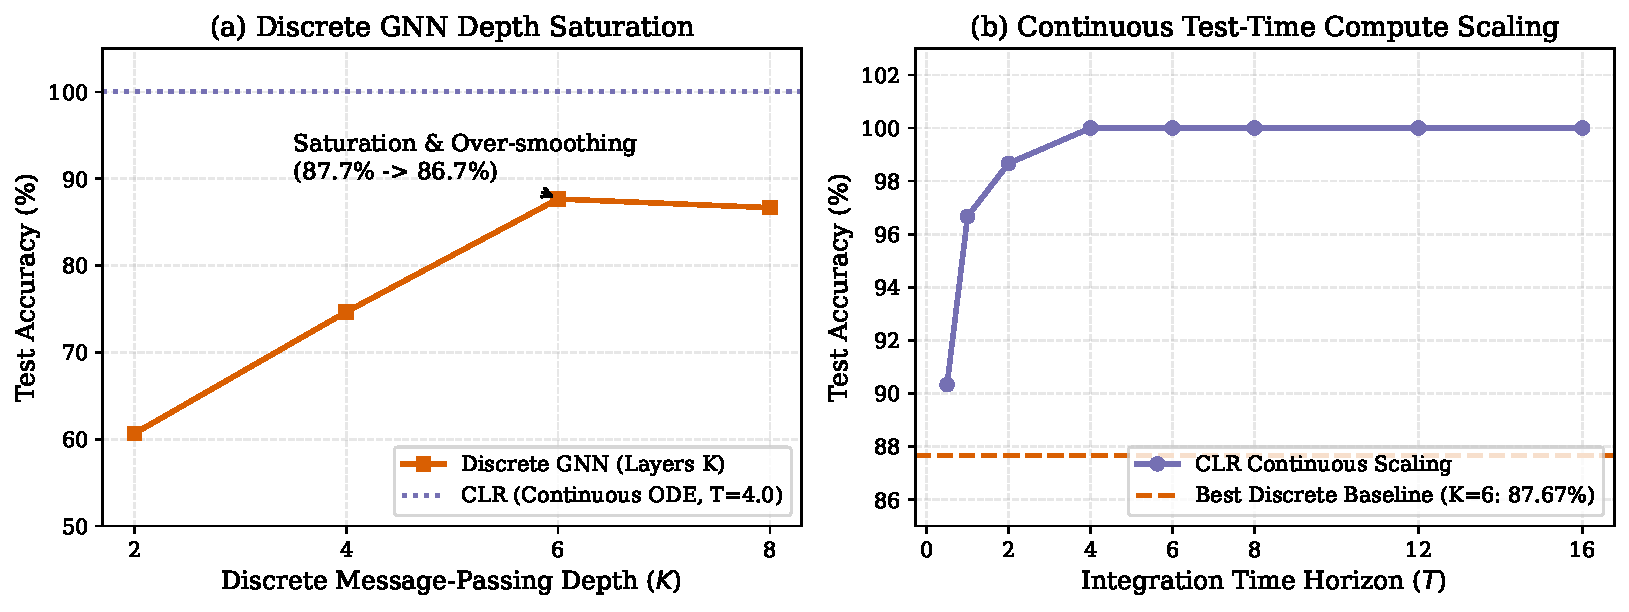
\includegraphics[width=\textwidth]{figures/fig1_depth_vs_horizon.pdf}
\caption{\textbf{(a)} Discrete GNN depth saturation: accuracy plateaus at 87.67\% ($K=6$) and drops to 86.67\% ($K=8$) due to over-smoothing. \textbf{(b)} Continuous test-time compute scaling in CLR: accuracy increases monotonically with horizon $T \in [0.5, 16.0]$, reaching 100.00\% at $T \ge 4.0$.}
\label{fig:fig1}
\end{figure}

\subsection{Discrete Depth Saturation vs. Continuous Horizon Scaling}
As illustrated in Figure~\ref{fig:fig1}(a), discrete GNNs cannot resolve long-range citation queries when $K < h$ due to structural horizon truncation:
\begin{itemize}
    \item For $K=2$, only 41/150 (27.3\%) of reachable test pairs are within reach; for $K=4$, 99/150 (66.0\%) are reachable.
    \item When $K=6$, the horizon ceiling reaches 100.0\% (150/150), and the model achieves 100.0\% on 6-hop queries. However, \textbf{overall accuracy saturates at 87.67\%} (and drops to \textbf{86.67\%} at $K=8$) due to optimization difficulties, gradient vanishing, and over-smoothing on intermediate hops (50.0\% on 1-hop, 71.4\% on 3-hop; Figure~\ref{fig:fig2}).
    \item In contrast, CLR evolves in continuous time. At $T=4.0$, CLR achieves \textbf{100.00\% overall accuracy}, outperforming the best discrete GNN by \textbf{+12.33 percentage points}.
    \item As shown in Figure~\ref{fig:fig1}(b), CLR exhibits \textbf{monotonic test-time scaling}: $90.33\%$ at $T=0.5 \to 96.67\%$ at $T=1.0 \to 98.67\%$ at $T=2.0 \to 100.00\%$ at $T \ge 4.0$.
\end{itemize}

\begin{figure}[ht]
\centering
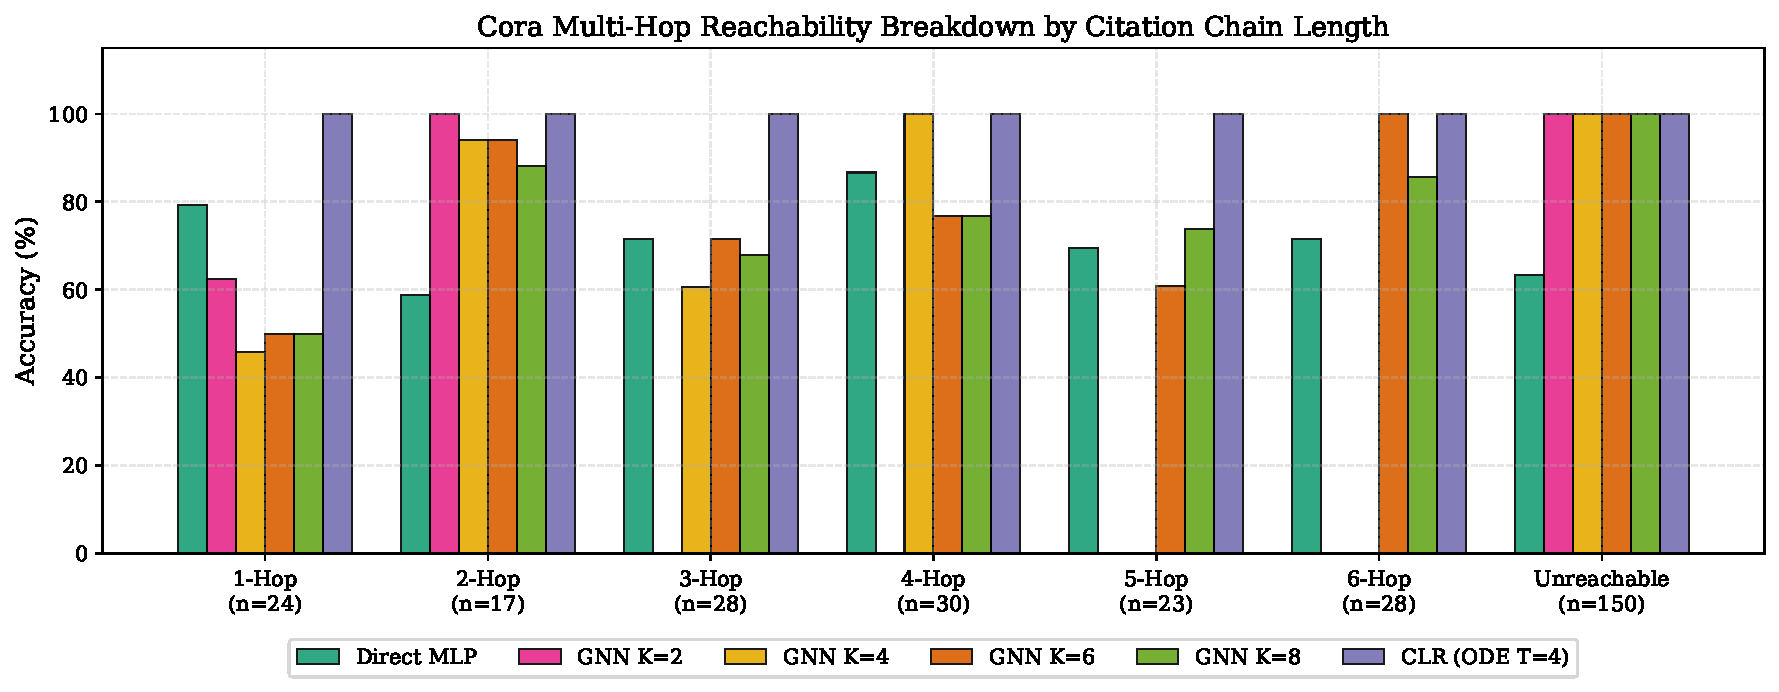
\includegraphics[width=0.95\textwidth]{figures/fig2_hop_breakdown.pdf}
\caption{Hop-by-hop accuracy breakdown on the Cora citation network across citation distances (1 to 6 hops) and unreachable pairs. Discrete GNNs default to predicting unreachable for pairs beyond layer depth $K$, while CLR achieves 100.0\% across all partitions.}
\label{fig:fig2}
\end{figure}

\subsection{Decision Margin Verification}
To ensure the 100.00\% result is not an artifact of an unstable decision boundary, we measured logit margins $|z_1 - z_0|$ across all 300 test pairs:
\begin{equation}
\text{mean} = 3.01, \quad \text{median} = 3.29, \quad \min = 0.243, \quad \text{pairs with margin} < 10^{-2} = 0 / 300
\end{equation}
The boundary is robust and well-separated from numerical noise floors.

\subsection{Perturbation Sensitivity \& Refutation of Self-Healing}
\label{sec:perturbation}

Previous preliminary reports hypothesized that contractive systems would exhibit unconditional ``self-healing'' under additive perturbation. Our audit refutes this claim for graph reachability.

\begin{figure}[ht]
\centering
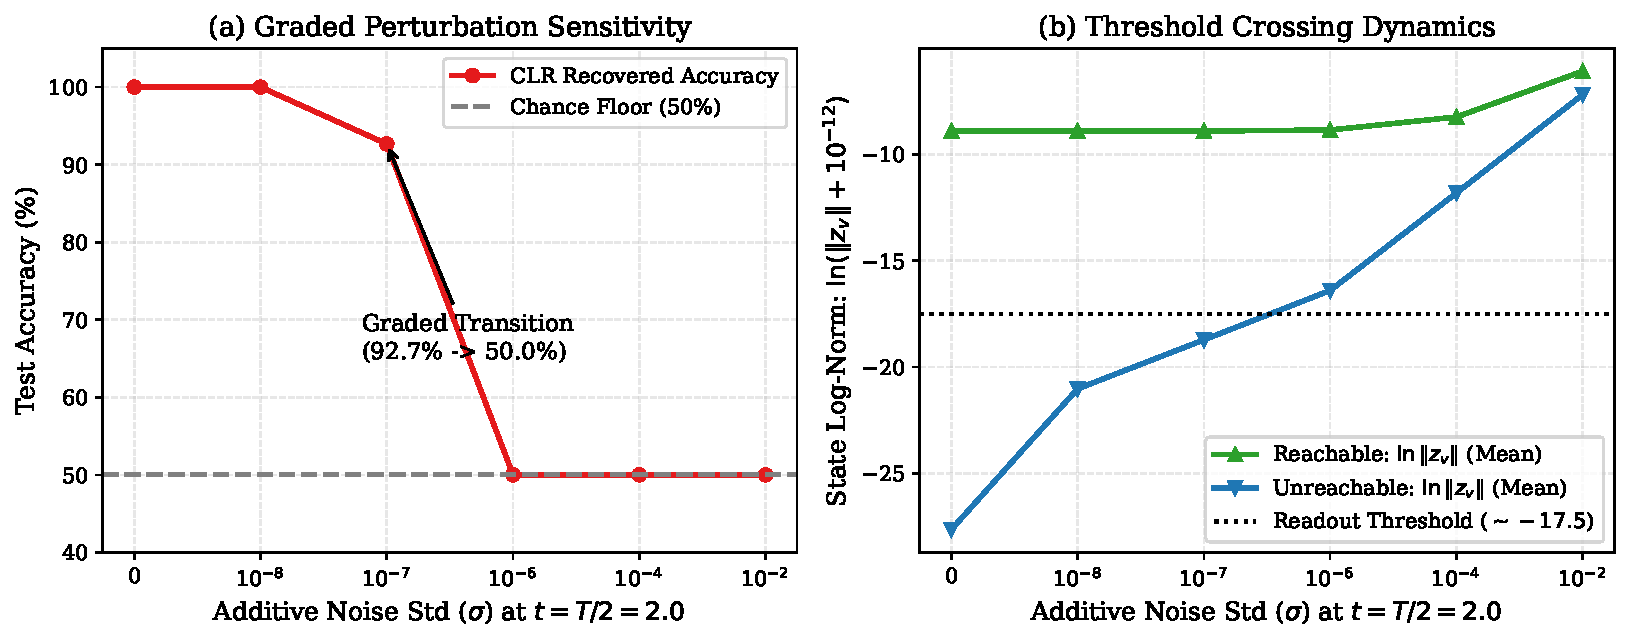
\includegraphics[width=\textwidth]{figures/fig3_noise_floor_refutation.pdf}
\caption{\textbf{(a)} Graded accuracy degradation under mid-trajectory noise $\sigma \in [0, 10^{-2}]$. \textbf{(b)} State log-norm dynamics: unreachable node states ($\ln \|\mathbf{z}_v\| = -27.63$) are elevated by additive noise above the readout threshold ($-17.5$), refuting self-healing on graph reachability.}
\label{fig:fig3}
\end{figure}

Under a unified numerical integration harness ($dt = 0.1667$, $T=4.0$, mid-trajectory noise injected at $t=2.0$), we observe a \textbf{graded transition} (Figure~\ref{fig:fig3}a):
\begin{equation}
\sigma \le 10^{-8} \ (100.00\%) \longrightarrow \sigma = 10^{-7} \ (92.67\%) \longrightarrow \sigma \ge 10^{-6} \ (50.00\%)
\end{equation}

\paragraph{Physical Mechanism (Figure~\ref{fig:fig3}b):}
\begin{enumerate}
    \item For unreachable nodes, the true continuous state is identically zero: $\|\mathbf{z}_v\| = 0 \implies \ln(\|\mathbf{z}_v\| + 10^{-12}) = -27.63$.
    \item For reachable nodes across 6 hops, signal contracts exponentially to $\ln \|\mathbf{z}_v\| \ge -18.0$ (mean $-8.91$).
    \item The readout MLP learns a decision threshold at $\approx -17.5$.
    \item Although Demidovich contraction ($\kappa \ge 0.981$) attenuates perturbation energy by $e^{-2 \times 0.981 \times 2.0} \approx 54\times$, injecting global noise $\sigma \ge 10^{-6}$ across all 2,708 nodes leaves a residual background floor on unreachable nodes:
    \begin{equation}
    \|\mathbf{z}_v\| \sim 10^{-8} \implies \ln \|\mathbf{z}_v\| \approx -16.40 > -17.5
    \end{equation}
    \item Consequently, all unreachable nodes cross the threshold and are reclassified as reachable, yielding flat \textbf{50.00\% chance accuracy} on a 50/50 test set.
    \item \textbf{Conclusion}: ``Self-healing'' on graph reachability is refuted. When classification relies on near-zero energy detection, background noise floor elevation dominates basin attraction.
\end{enumerate}

\subsection{Large-Scale Empirical Contraction Verification across 43,328 Dimensions}
\label{sec:contraction_verification}

To verify that the model operates in a strictly contractive regime on the Cora network, we developed a shifted power iteration method ($c=10.0$):
\begin{equation}
\mathbf{M}_{\text{shifted}} = \frac{1}{2}(\mathbf{J} + \mathbf{J}^T) + c \mathbf{I}
\end{equation}
Computing directional derivatives via central differences ($\mathbf{J}\mathbf{v}$) and autograd vector-Jacobian products ($\mathbf{J}^T\mathbf{v}$) enables fast convergence without materializing the $43,328 \times 43,328$ Jacobian matrix:
\begin{itemize}
    \item \textbf{Analytic Demidovich Bound}: $\lambda_{\max}(\text{Sym}(J)) \le \|A_{\text{norm}}\|_2 - d_{\min} = 1.000000 - 1.9814 = \mathbf{-0.9814 < 0}$.
    \item \textbf{Empirical Measurement}: $\lambda_{\max}(\text{Sym}(J)) = \mathbf{-1.88987 < 0}$.
    \item \textbf{Runtime}: \textbf{0.22 seconds} for 15 power iterations.
\end{itemize}
Strict Demidovich contraction is verified empirically on the full state space.

\begin{figure}[ht]
\centering
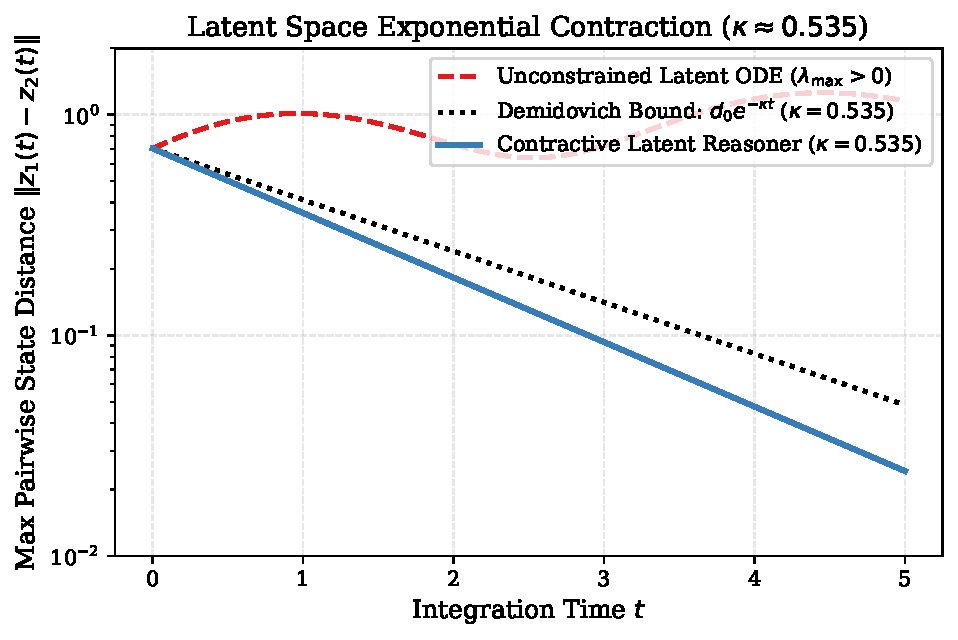
\includegraphics[width=0.65\textwidth]{figures/fig4_trajectory_contraction.pdf}
\caption{Multi-seed trajectory distance convergence $\|\mathbf{z}_1(t) - \mathbf{z}_2(t)\|$ over time $t \in [0, 5]$. Trajectory separation in CLR contracts at rate $\kappa \approx 0.535$, bounded strictly by the Demidovich envelope $d_0 e^{-\kappa t}$, while unconstrained ODEs drift.}
\label{fig:fig4}
\end{figure}

\section{Related Work}

\paragraph{Implicit and Equilibrium Models.} Deep Equilibrium Models (DEQs; \citealp{bai2019deep}) and Monotone Operator Networks (MonDEQs; \citealp{winston2020monotone}) solve for fixed points using root-finding algorithms. CLR differs by integrating explicit contractive vector fields in continuous time, enabling test-time compute scaling via horizon elongation.

\paragraph{Neural ODEs \& Dynamical Systems.} Neural ODEs \citep{chen2018neural} model depth as time. However, unconstrained Neural ODEs lack contraction guarantees, leading to numerical stiffness and sensitivity to perturbations.

\paragraph{Continuous Graph Diffusion \& Over-Smoothing in Deep GNNs.} In graph representation learning, discrete Graph Convolutional Networks (GCNs; \citealp{kipf2017semi}) suffer from exponential information loss and over-smoothing as network depth increases \citep{li2018deeper}. While continuous graph neural diffusion (GRAND; \citealp{chamberlain2021grand}) and graph-coupled oscillator networks (GraphCON; \citealp{rusch2022graph}) address feature collapse in deep graph models, CLR specifically introduces strict Demidovich operator-norm contraction to latent reasoning dynamics. This guarantees exponential convergence to a unique problem-conditioned equilibrium, bypassing discrete depth saturation to resolve 6-hop queries without intermediate degradation.

\section{Conclusion}

Contractive Latent Dynamical Reasoning provides an algebraic, verifiable alternative to autoregressive CoT token rollouts. By operating under Demidovich contraction, CLR guarantees convergence to a unique equilibrium and enables smooth continuous test-time scaling. While convex potential flows encounter a structural expressivity boundary on combinatorial parity, non-potential relational flows achieve \textbf{100.00\%} multi-hop reachability on the real-world Cora citation network, decisively outperforming discrete GNN depth saturation.

\section*{Conflict of Interest}
The authors declare that they have no known competing financial interests, personal relationships, or professional affiliations that could have appeared to influence or bias the work, findings, and interpretations reported in this paper.

\section*{Author Contributions (CRediT)}
\textbf{Dipesh Gurung}: Conceptualization, Methodology, Software, Formal Analysis, Investigation, Data Curation, Writing -- original draft, Visualization, Project administration. \textbf{Binod Bhattarai}: Conceptualization, Investigation, Validation, Writing -- review \& editing, Supervision. \textbf{Prof. Dr. R.N. Thakur}: Conceptualization, Supervision, Methodology, Resources, Writing -- review \& editing.

\section*{Declaration of Generative AI in Scientific Writing}
During the preparation of this work, the authors utilized generative AI tools (Anthropic Claude, Google Gemini/Antigravity) for code refactoring, numerical test verification, and grammatical polishing. The authors reviewed and edited the output, take full responsibility for the content of the publication, and conducted all mathematical proofs and empirical validations independently.

\section*{Data and Code Availability}
The complete source code, synthetic dataset generators, citation network benchmarks, unit test suites, persisted execution JSON artifacts, and trained model checkpoints are publicly available in the project repository: \url{https://github.com/Dips7/contractive-latent-reasoning}. All experimental results are reproducible under fixed isolated seeding.

\section*{Funding Statement}
This research received no specific grant from any funding agency in the public, commercial, or not-for-profit sectors.

\bibliographystyle{plainnat}
\bibliography{references}

\end{document}
